\section{Experiments}
\label{sec:experiments}

\subsection{Dataset}
\label{subsec:dataset}
Due to its commercial value, real-life SC systems such as Uber and TaskRabbit do not make their datasets available to public. However, we were able to use a large collection of geo-tagged images from Flickr \cite{Thomee15} as an input to Auction-SC. The dataset consists of \textasciitilde 15 million images with attributes such as location, time taken, time uploaded, the user who took the picture, etc.

We correspond each image with a spatial task considering that the task was to take a photo at a specific location. We set the deadline of the task to the time the image was taken and the duration of the task to the interval between the time the image was taken and the time it was uploaded. Each user in the dataset corresponds to a worker. The original location of the worker is randomly selected. The worker is available in the interval between the first time he took a photo and the last time he uploaded one. We ran 5 separate instances, each of which with images of a different metropolitan area. \cref{tab:flickr_stats} shows the total number of tasks (and workers) for each city. 

\begin{table}[h]
\begin{center}
\begin{tabular}{| l || c | c |} \hline
			&	\# of Tasks	&	\# of Workers	\\ \hline
Los Angeles	&	219,332		&		19,081		\\ \hline
New York	&	390,229		&		17,603		\\ \hline
London		& 	366,034		&		18,480		\\ \hline
Paris		&	237,344		&		14,275		\\ \hline
Beijing		&	23,335		&		1,598		\\ \hline
\end{tabular}
\caption{\small{Number of tasks/worker for each city in Flickr dataset}}
\label{tab:flickr_stats}
\end{center}
\end{table}

We also generated a synthetic dataset with realistic streaming workload based on the methodology proposed in \cite{Tang07}. To generate a workload suitable for SC systems we modeled three different sets of parameters:

\vspace{0.1in}
\noindent \textbf{Temporal Parameters:} In \cite{Basu15}, it is shown that in crowdsourcing environments, workers and tasks arrive following Poisson processes \cite{Stoyan87}.The default Poisson arrival rates for tasks and workers are $\mu_t = 20/min$ and $\mu_w = 3/min$ respectively. Subsequently, the duration of the tasks and workers were randomly sampled from closed range of $\left[1,4 \right]$ hours and $\left[1,8 \right]$ hours respectively.

\vspace{0.1in}
\noindent \textbf{Spatial Parameters:} \cref{fig:la_flickr} shows the spatial distribution of tasks from our real world dataset in Los Angeles. As depicted the tasks are not uniformly distributed in space. The spatial distribution is rather skewed, meaning that the density of the tasks in certain areas is higher. To model the same behavior in our synthetic workload, we created 6 two dimensional Gaussian clusters with randomly selected means and standard deviations. Eighty percent of the tasks are sampled within the clusters and the rest are uniformly distributed.

\vspace{0.1in}
\noindent \textbf{Static Parameters:} In addition to the spatiotemporal parameters, we consider two other parameters. The default \emph{workload size} of each experiment is 10K tasks. The task arrival rate and the number of tasks determine the duration of the simulation. Based on the duration of the simulation and the worker arrival rate, the total number of workers may vary.\\
The maximum number of tasks a worker can perform, i.e., $w_{max}$, is a uniformly random number from the closed interval $\left[8,12 \right]$.

\begin{figure}[h]
	\centering
	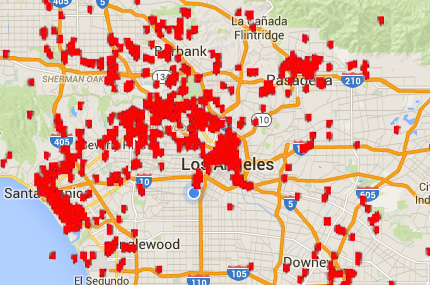
\includegraphics[scale=0.4]{figures/la_flickr.jpg}
	\caption{Spatial Distribution of Tasks in Flickr}\label{fig:la_flickr}
\end{figure}

\subsection{Online vs. Offline}
\vspace{0.1in}
In the first set of experiments, we compare how the results of the real-time algorithms compare with the optimal solution computed using the offline clairvoyant algorithm explained in \cref{sec:exactalgo}. Because of the high complexity of the offline algorithm, we are not able to run tests with large workloads and thus we use workloads with 100 tasks. The experimental results in \cref{fig:off_vs_on} show that the best real-time algorithm perform \textasciitilde 60\% of the optimal solution. Our results are consistent with studies that compute a \emph{competitive ratio} \cite{Sleator85} of $1 - e^{-1}$ for the online matching problem with random inputs \cite{Goel08}.

\begin{figure}[h]
	\centering
	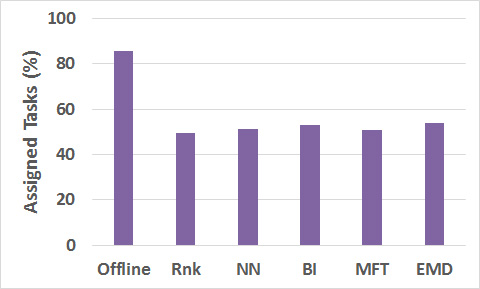
\includegraphics[width = 0.6\columnwidth]{figures/off_vs_on.jpg}
	\caption{Comparison of Offline and Real-time approaches}\label{fig:off_vs_on}
\end{figure}

\vspace{0.2in}
\subsection{Assignment Quality}
In this section we evaluate the quality of the assignments using different real-time non-clairvoyant algorithms. First, we compare them using the Flickr and the synthetic datasets. Subsequently, using the synthetic datasets, we show how the spatial and temporal settings of the problem can affect the performance of the real-time assignment quality.

\begin{figure}[h]
    \centering
    \subfigure[Flickr]{
        \label{fig:quality_real}
        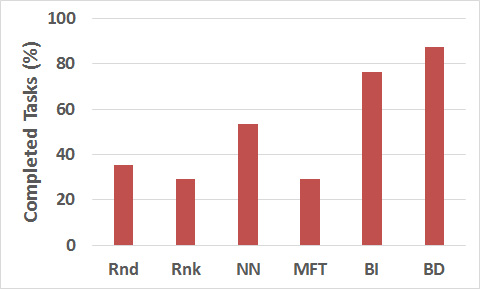
\includegraphics[width = 0.45\columnwidth]{figures/quality_real.jpg}
    }
    \subfigure[Synthetic]{
        \label{fig:quality_syn}
        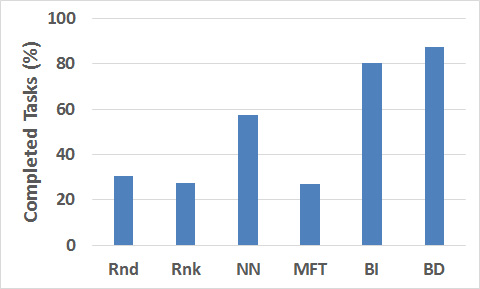
\includegraphics[width = 0.45\columnwidth]{figures/quality_syn.jpg}
    }
    \caption{Assignment Quality of Real-Time Approaches}
    \label{fig:quality}
\end{figure}

\cref{fig:quality} compares the assignment quality of different real-time algorithms. As we can see, both SC approaches outperforms the best non-SC algorithm by more than 25\%. The main reason as explained in \cref{sec:onlinealgo} is that, the SC rules performs scheduling when assigning tasks to workers. Furthermore, the BD approach outperforms BI by at most 10\%. This is not surprising as BD tends to "move" workers to areas where future tasks are more likely to appear, thus achieving higher assignment in long term. Among the non-SC approaches NN outperforms other rules by almost 2 times more completed tasks. The reason MFT does not outperform baseline approaches (Rnd and Rnk) can be explained by what we call a \emph{radical move}. A \emph{radical move} is when the SC-Server assigns a task to a worker which requires it to move a relatively long distance to reach the location of that task. Since we do not consider any spatial proximity to the task with MFT, there is a high chance to end up with assignments resulting in radical moves. With NN and BI the general idea is to prevent radical moves as much as possible. With BD, although radical moves occur, but only if the worker moves to areas where there will be more tasks to complete. 

\begin{figure}[h]
    \centering
    \subfigure[Rnd]{
        \label{fig:rnd_comp}
        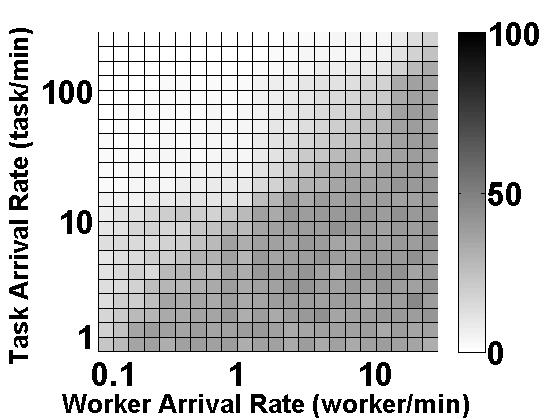
\includegraphics[width = 0.45\columnwidth]{figures/rnd.jpg}
    }
    \subfigure[Rnk]{
        \label{fig:rnk_comp}
        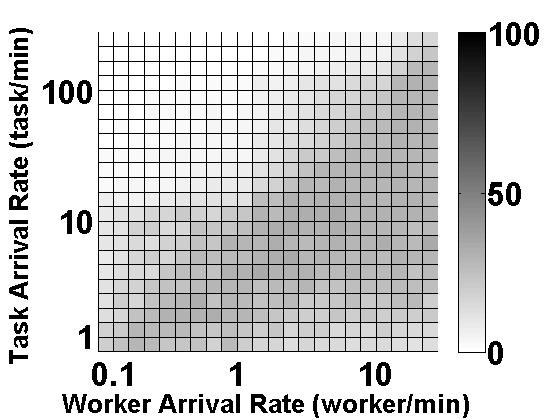
\includegraphics[width = 0.45\columnwidth]{figures/rnk.jpg}
    }
    \subfigure[MFT]{
        \label{fig:mft_comp}
        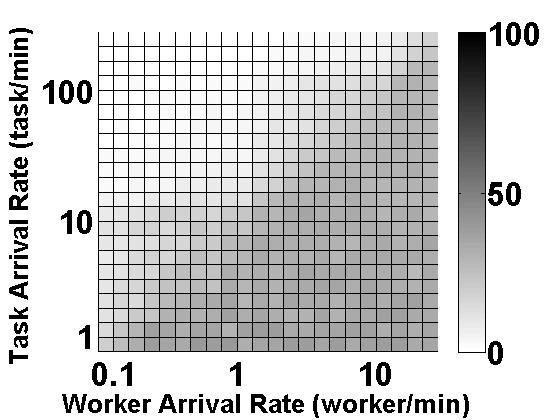
\includegraphics[width = 0.45\columnwidth]{figures/mft.jpg}
    }
    \subfigure[NN]{
        \label{fig:nn_comp}
        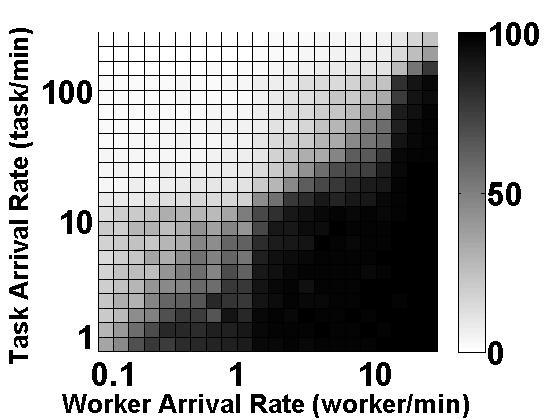
\includegraphics[width = 0.45\columnwidth]{figures/nn.jpg}
    }
    \subfigure[BI]{
        \label{fig:bi_comp}
        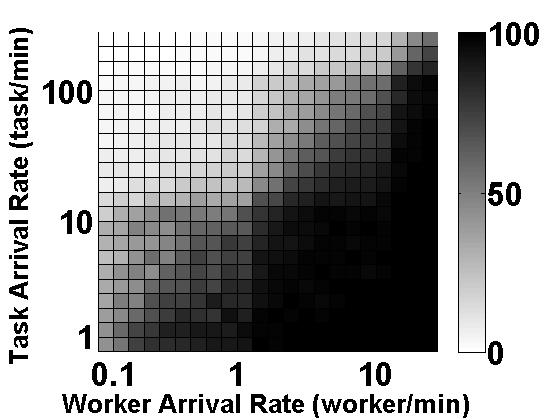
\includegraphics[width = 0.45\columnwidth]{figures/bi.jpg}
    }
    \subfigure[BD]{
        \label{fig:emd_comp}
        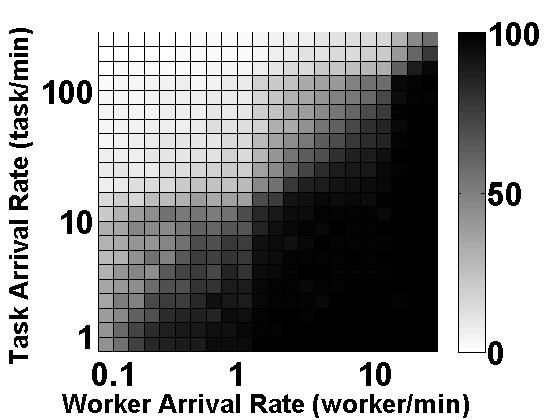
\includegraphics[width = 0.45\columnwidth]{figures/emd.jpg}
    }
    \caption{\small{Assignment Profile-Varying Worker/Task Arrival Rates}}
    \label{fig:tw_rate}
\end{figure}

In order to study the effect of temporal parameters in SC, we ran several experiments using different pairs of task arrival rate ($t_{rate}$ and worker arrival rate ($w_{rate}$). In \cref{fig:tw_rate} we show the effect of increasing $t_{rate}$ and $w_{rate}$ on the quality of the assignment. The level of grayness corresponds to the percentage of completed tasks with black and white representing 100\% and 0\% respectively. As we can see with small number of workers, as we increase the task arrival rate, the percentage of completed tasks decreases where at the top left corner of each plot we get close to 0\%. On the other hand in \cref{fig:nn_comp,fig:bi_comp,fig:emd_comp} for NN, BI and BD, with small number of incoming tasks, as we increase $w_{rate}$ eventually all tasks will be completed. \cref{fig:tw_rate} clearly shows that NN, BI and BD outperform Rnd, Rnk and MFT independent of the $t_{rate}$ and $w_{rate}$.

\begin{figure}[h]
	\centering
	\subfigure[BI Vs. NN]{
        \label{fig:bi_nn}
        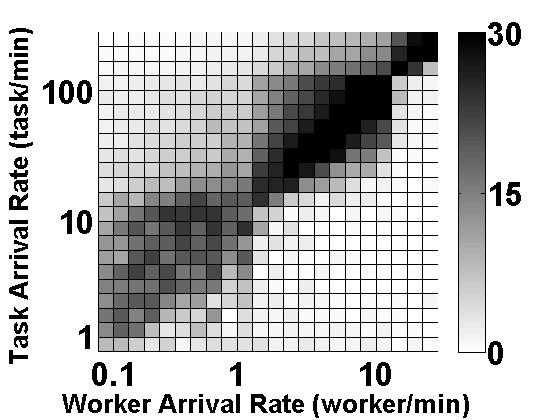
\includegraphics[width = 0.45\columnwidth]{figures/bi_nn.jpg}
    }
    \subfigure[BD Vs. NN]{
        \label{fig:emd_nn}
        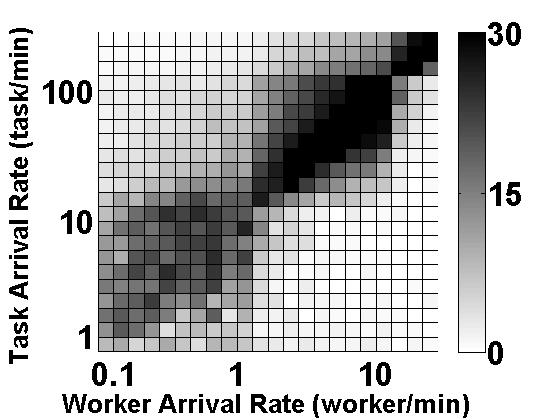
\includegraphics[width = 0.45\columnwidth]{figures/emd_nn.jpg}
    }
    \subfigure[BD Vs. BI]{
        \label{fig:emd_bi}
        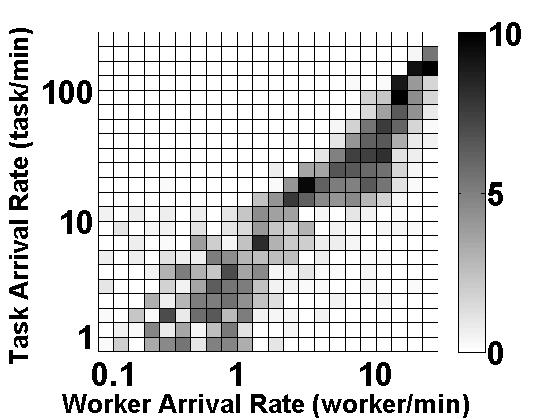
\includegraphics[width = 0.45\columnwidth]{figures/emd_bi.jpg}
    }
	\caption{\small{Assignment Difference-Varying Worker/Task Arrival Rates}}\label{fig:rate_comp}
\end{figure}

To better evaluate the leading real-time approaches, NN, BI and BD, in \cref{fig:rate_comp} we performed a pair-wise comparison by taking their task completion rates. For example, \cref{fig:bi_nn} shows the difference between BI and NN. We observe that these three approaches perform similarly in the two extreme cases discussed in \cref{fig:tw_rate}, i.e., high task-low worker nad low task-high worker. BI and BD outperform NN up to 30\% when the problem is more complex, i.e., outside the extreme cases. An interesting observation in \cref{fig:bi_nn,fig:emd_nn} is that BI and BD outperform NN by a much larger margin at scale (higher $t_{rate}$ and $w_{rate}$). The reason is that with higher higher $t_{rate}$ and $w_{rate}$ more workers are moving around and more tasks come and leave so in general the spatiotemporal dynamism of the system increases. BI and BD cope with the dynamism by guaranteeing a task gets assigned to worker that can complete it. On the contrary, NN ignores the schedule of the worker during assignment and this becomes more important as there is more dynamism in the system.

\begin{figure}[h]
	\centering
	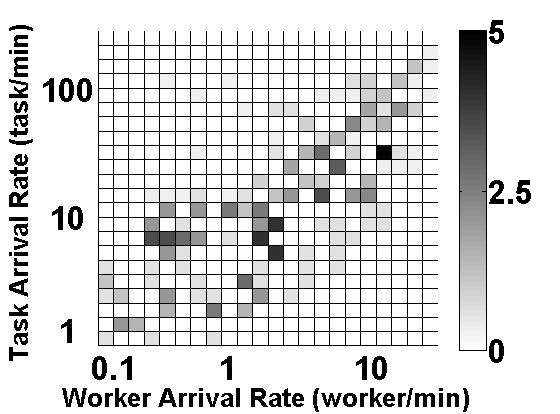
\includegraphics[scale=0.25]{figures/bi_abi.jpg}
	\caption{Assignment Difference of BI Vs. ApproxBI}\label{fig:bi_abi}
\end{figure}

We mentioned earlier that with the SC-rules, the workers perform an exhaustive search to find out if they can fit a new task into their schedule. As workers accept new tasks, they also complete some other tasks so as we observed in our experiments, performing an exhaustive search did not cause any scalability issues. Nevertheless, one might want to replace the exhaustive search with an approximate algorithm with polynomial run-time. in ApproxBI, we use the algorithm in \cite{Rosenkrantz74} that runs in $O(n^2)$. \cref{fig:bi_abi} shows the change affects the quality of the assignment by less than 5\%. The difference caused by ApproxBI is that the workers that are eligible for a task using BI, may not be able to fit the task in their schedules using ApproxBI due to the approximation. As a result, using ApproxBI the server may not be able to assign some tasks even if they can be completed using BI. Fortunately, as shown in \cref{fig:bi_abi}, that does not happen very often regardless of $t_{rate}$ and $w_{rate}$.

\subsection{Scalability}
The last set of experiments focus on measuring the scalability of two system architectures, i.e., centralized and Auction-SC (decentralized). We compare the scalability of the real-time Auction-SC algorithms with the equivalent implementation of the same algorithms on a single centralized SC-Server. 

In practice, a real-time SC system (either Auction-SC or centralized) works similar to a \emph{complex event processing (CEP)} engine \cite{Luckham01}. We can measure the scalability of such systems by their throughput: the number of tasks processed per second , or equivalently, the processing time per task, shown in \cref{fig:runtime}. Because of the decentralized architecture of Auction-SC, in \cref{fig:runtime} we see that the average processing time of a single task does not change as the arrival rate of workers increases. On the contrary, with the centralized architecture, the average processing time of a single task increases linearly as we increase the number of workers and in several orders of magnitude higher than Auction-SC approaches. Although BD consumes more time than other real-time algorithms, but only takes \textasciitilde 3 milliseconds.

\begin{figure}[h]
    \centering
    \subfigure[\emph{\small{wRate = 1 worker/min}}]{
        \label{fig:runtime_50}
        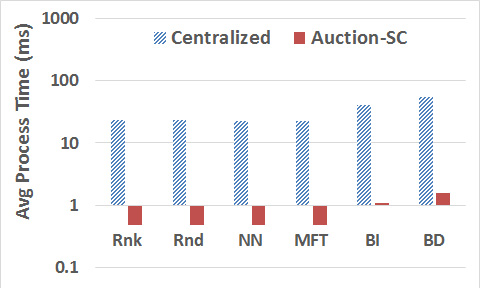
\includegraphics[width = 0.45\columnwidth]{figures/run_time_50.jpg}
    }
    \subfigure[\emph{\small{wRate = 2 worker/min}}]{
        \label{fig:runtime_100}
        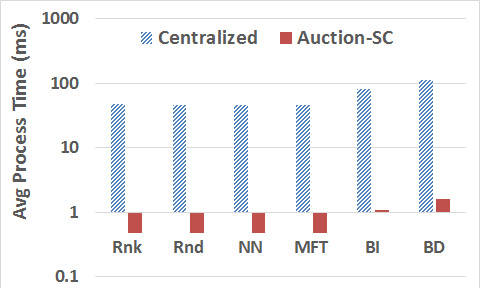
\includegraphics[width = 0.45\columnwidth]{figures/run_time_100.jpg}
    }
    \subfigure[\emph{\small{wRate = 4 worker/min}}]{
        \label{fig:runtime_200}
        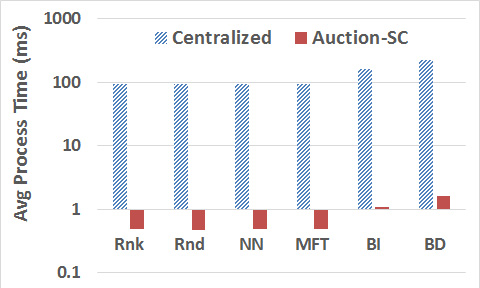
\includegraphics[width = 0.45\columnwidth]{figures/run_time_200.jpg}
    }
    \subfigure[\emph{\small{wRate = 8 worker/min}}]{
        \label{fig:runtime_400}
        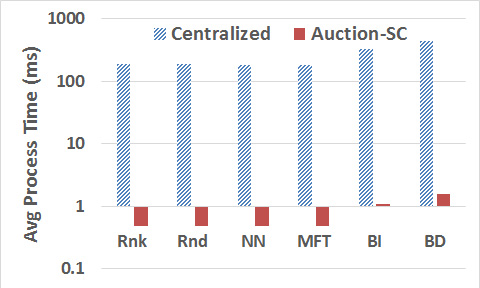
\includegraphics[width = 0.45\columnwidth]{figures/run_time_400.jpg}
    }
       \vspace{-0.15in}
    \caption{Average processing time for a single task}
    \label{fig:runtime}
\end{figure}

For a \emph{CEP} engine, it is also common to measure the queuing delay of events \cite{Wu06} once they arrive in the system as a metric for how scalable the systems is. In \cref{fig:queue} we compare the average queuing delay of tasks between running the two architectures after running for 1 hour. We can see that the centralized system suffers from queuing delays with less than 10 tasks/second. On the other hand, with Auction-SC, even for BD, we do not observe queuing delays for up to 500 tasks/second. \cref{fig:queue_auc} also shows that BD incurs higher delay than BI but results in higher completion rates, as in \cref{fig:quality,fig:rate_comp}. Users of Auction-SC can choose between BD and BI to balance their needs for assignment quality and efficiency.

\begin{figure}[h]
    \centering
    \subfigure[\emph{\small{Centralized}}]{
        \label{fig:queue_cent}
        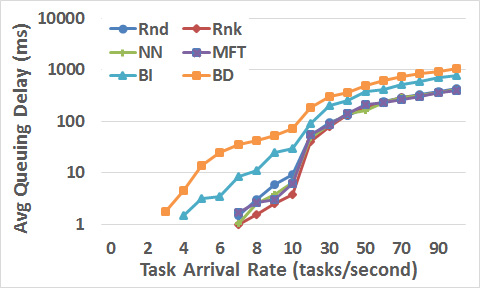
\includegraphics[width = 0.65\columnwidth]{figures/queue_cent.jpg}
    }
    \subfigure[\emph{\small{Auction-SC}}]{
        \label{fig:queue_auc}
        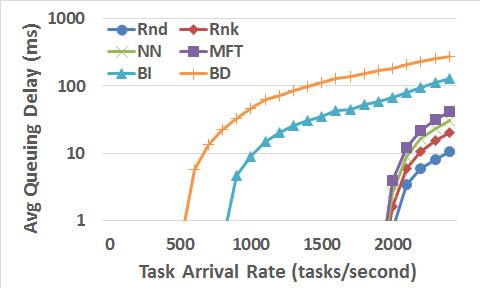
\includegraphics[width = 0.65\columnwidth]{figures/queue_auc.jpg}
    }
    \vspace{-0.15in}
    \caption{Average queuing delay}
    \label{fig:queue}
\end{figure}

To summarize the results of our experiments, we showed that when SC bidding rules are used, the quality of the assignment is much higher as compared to when a non-SC rule is used. The consideration of scheduling at the time a task is being assigned is the main reason for the better assignments. When running on a single centralized SC-Server, neither one of bidding rules can scale. The time required to process a single task increases linearly as more workers are added to the system. Scalability on a centralized single server suffers more when SC bidding rules are used due to their higher computation complexity. However, with Auction-SC we solve the scalability problem by splitting the scheduling and assignment responsibilities between workers and the SC-Server. Consequently, Auction-AC can afford to execute complex SC bidding rules, resulting in a very high quality assignment. \cref{tab:summary} shows the summary of our experimental results.

\begin{table*}
  \centering
  \begin{tabular}{|c|c|c|c|c|c|c|c|c|}
    \hline
    \multicolumn{2}{|>{\columncolor{kugray5}}c|}{}&\multicolumn{4}{c|}{non-SC bidding rules}&\multicolumn{2}{c|}{SC bidding rules}\\
    \arrayrulecolor{kugray5}
    \arrayrulecolor{black}
    \cline{3-8}
    \multicolumn{2}{|>{\columncolor{kugray5}}c|}{}&Rnd&Rnk&NN&MFT&BI&BD\\
    \hline
    \multirow{2}{*}{Centralized}&Scalability&Bad&Bad&Bad&Bad&Very Bad&Very Bad\\
    \cline{2-8}
                         		&Assignment Quality&Very Bad&Very Bad&Bad&Very Bad&Very Good&Very Good\\
    \hline
    \multirow{2}{*}{Auction-SC}&Scalability&Very Good&Very Good&Very Good&Very Good&Good&Good\\
    \cline{2-8}
                         		&Assignment Quality&Very Bad&Very Bad&Bad&Very Bad&Very Good&Very Good\\
    \hline
  \end{tabular}
  \caption{Summary of Experimental Results}
  \label{tab:summary}
\end{table*}